\documentclass[main.tex]{subfiles}

\begin{document}

\chapter{Methodology}

\section{Spline evaluation}
A B-spline function is a combination of flexible bands that is controlled by a number of points that are called control points, creating smooth curves.\\

A B-spline of order $n$ is a piece wise polynomial function of degree {$n−1$}  in a variable x . It is defined over n+1  locations  {$t_{j}$}, called knots or breakpoints, which must be in non-descending order  { $t_{j}\leq t_{j+1}$}. The B-spline contributes only in the range between the first and last of these knots, and is zero elsewhere.\\


Periodic B-spline is a special case of B-spline where we duplicate the first $k-1$ control points, at the end.

\begin{figure}[H]
    \centering
    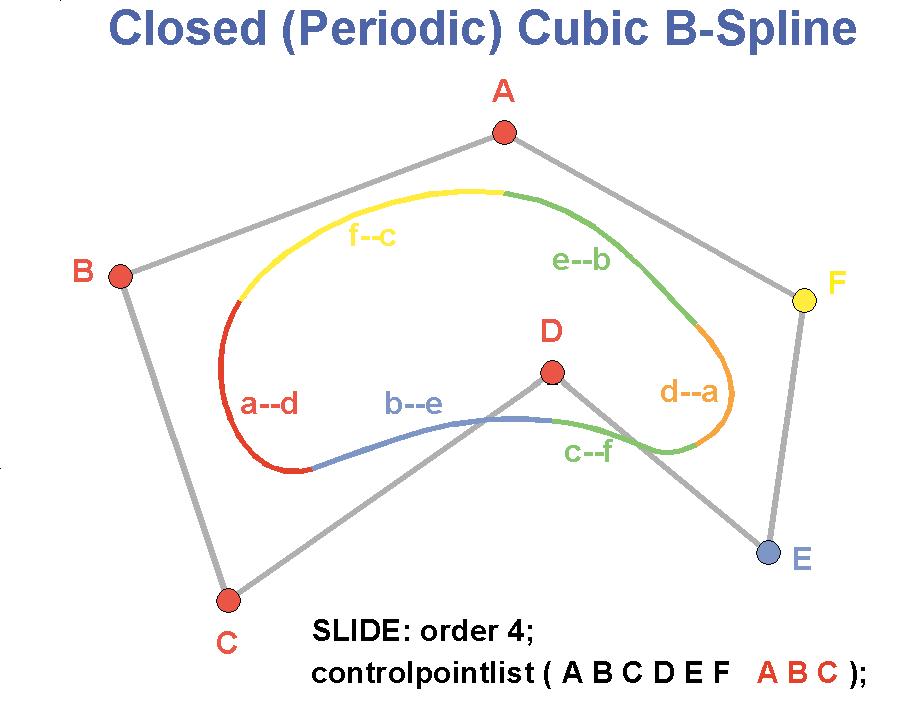
\includegraphics[width=10cm]{presentationImages/BsplineLocality.png}
    \caption{Image showcasing the Locality property of the Periodic B-Spline}
\end{figure}


In order to evaluate the B-Spline at any point we use de Boor's algorithm, which is an efficient and numerically stable scheme.\\

% The usefulness of B-splines lies in the fact that any spline function of order n on a given set of knots can be expressed as a linear combination of B-splines: 
\begin{equation}
    S(x) = \sum_{i}^{n-1}C_{i}\phi_{i, k}(x)
\end{equation}

\begin{align}
    \phi_{i, 0}(x) = \begin{cases}
      1 & \text{if $t_i \leq x \leq t_{i+1}$}\\
      0 & \text{Otherwise}
      \end{cases}
\end{align}

\begin{equation}
    \phi_{i, k}(x) = \frac{x - t_i}{t_{i+p} - t_i}\phi_{i, k-1}(x) + \frac{t_{i+p+1} - x}{t_{i+p+1} - t_{i+1}}\phi_{i+1, k-1}(x)
\end{equation}
Where : $\phi_{i, k}(x)$ is the i-th spline basis  function of degree k evaluated at the point x. $t_i$ is the ith knot. x is the parametrization .\\

To accelerate training, we set a contour sample size, and construct a precomputed sampling matrix having a shape of (NumSamples=n x numControlPoints=m).
We pick uniformly distributed knot vector from the interval (1/m to (m+1)/m).Basically we evaluate the B-spline basis function on each couple (parametrization, knot) thus reducing the sampling to a single dot operation for the entire batch.


\begin{equation}
\begin{pmatrix}
    S_x^0  & S_y^0 \\
    \vdots & \vdots\\
    S_x^m  & S_y^m \\
    \end{pmatrix} = 
    \begin{pmatrix}
        \phi_0^{k}(x_0) & \dots & \phi_m^{k}(x_0)\\
        \vdots & \ddots & \vdots \\
        \phi_0^{k}(x_n) &\dots  & \phi_m^{k}(x_n)
    \end{pmatrix}
    \begin{pmatrix}
    C_x^0  & C_y^0 \\
    \vdots & \vdots\\
    C_x^m  & C_y^m \\
    \end{pmatrix}
\end{equation}


\section{Model}
The model is made of 2 stages. The first one called the encoder, the second one consist of multiple branch each computing a certain component.

The first component is the object probabilities (which will serve as a score to pick the most probable instances). The second component Will predict the actual control points that define the shape of the instance for each pixel, which are defined by a pair (Distance, and angle expressed in relative polar coordinates) for each control point. The third component predict the probability of overlap between instances, which will later help build a posterior probability for sampling instances. 

\begin{figure}[H]
    \centering
    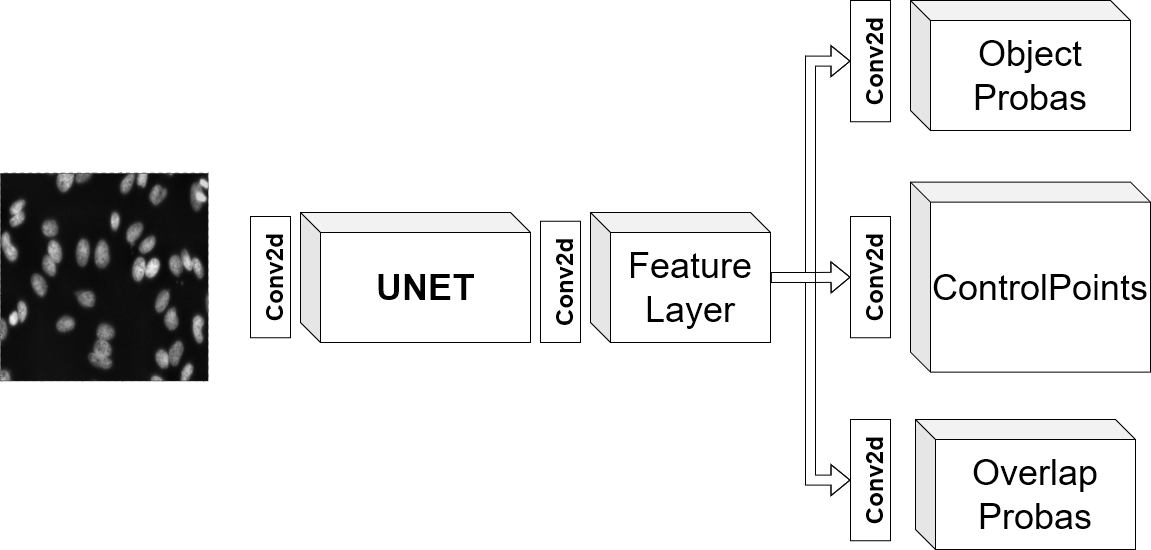
\includegraphics[width=15cm]{presentationImages/splinedistModel.png}
    \caption{The global architecture of the model}
\end{figure}


In particular the ControlPoints branch is composed of 2 branches, (One predicting the angles, and the other the distances), these are converted first to Cartesian coordinates , then converted from relative coordinates to image coordinates by adding a shift value corresponding to the location of the pixel. As a last step, we duplicate the first $k-1$ control points

\begin{figure}[H]
    \centering
    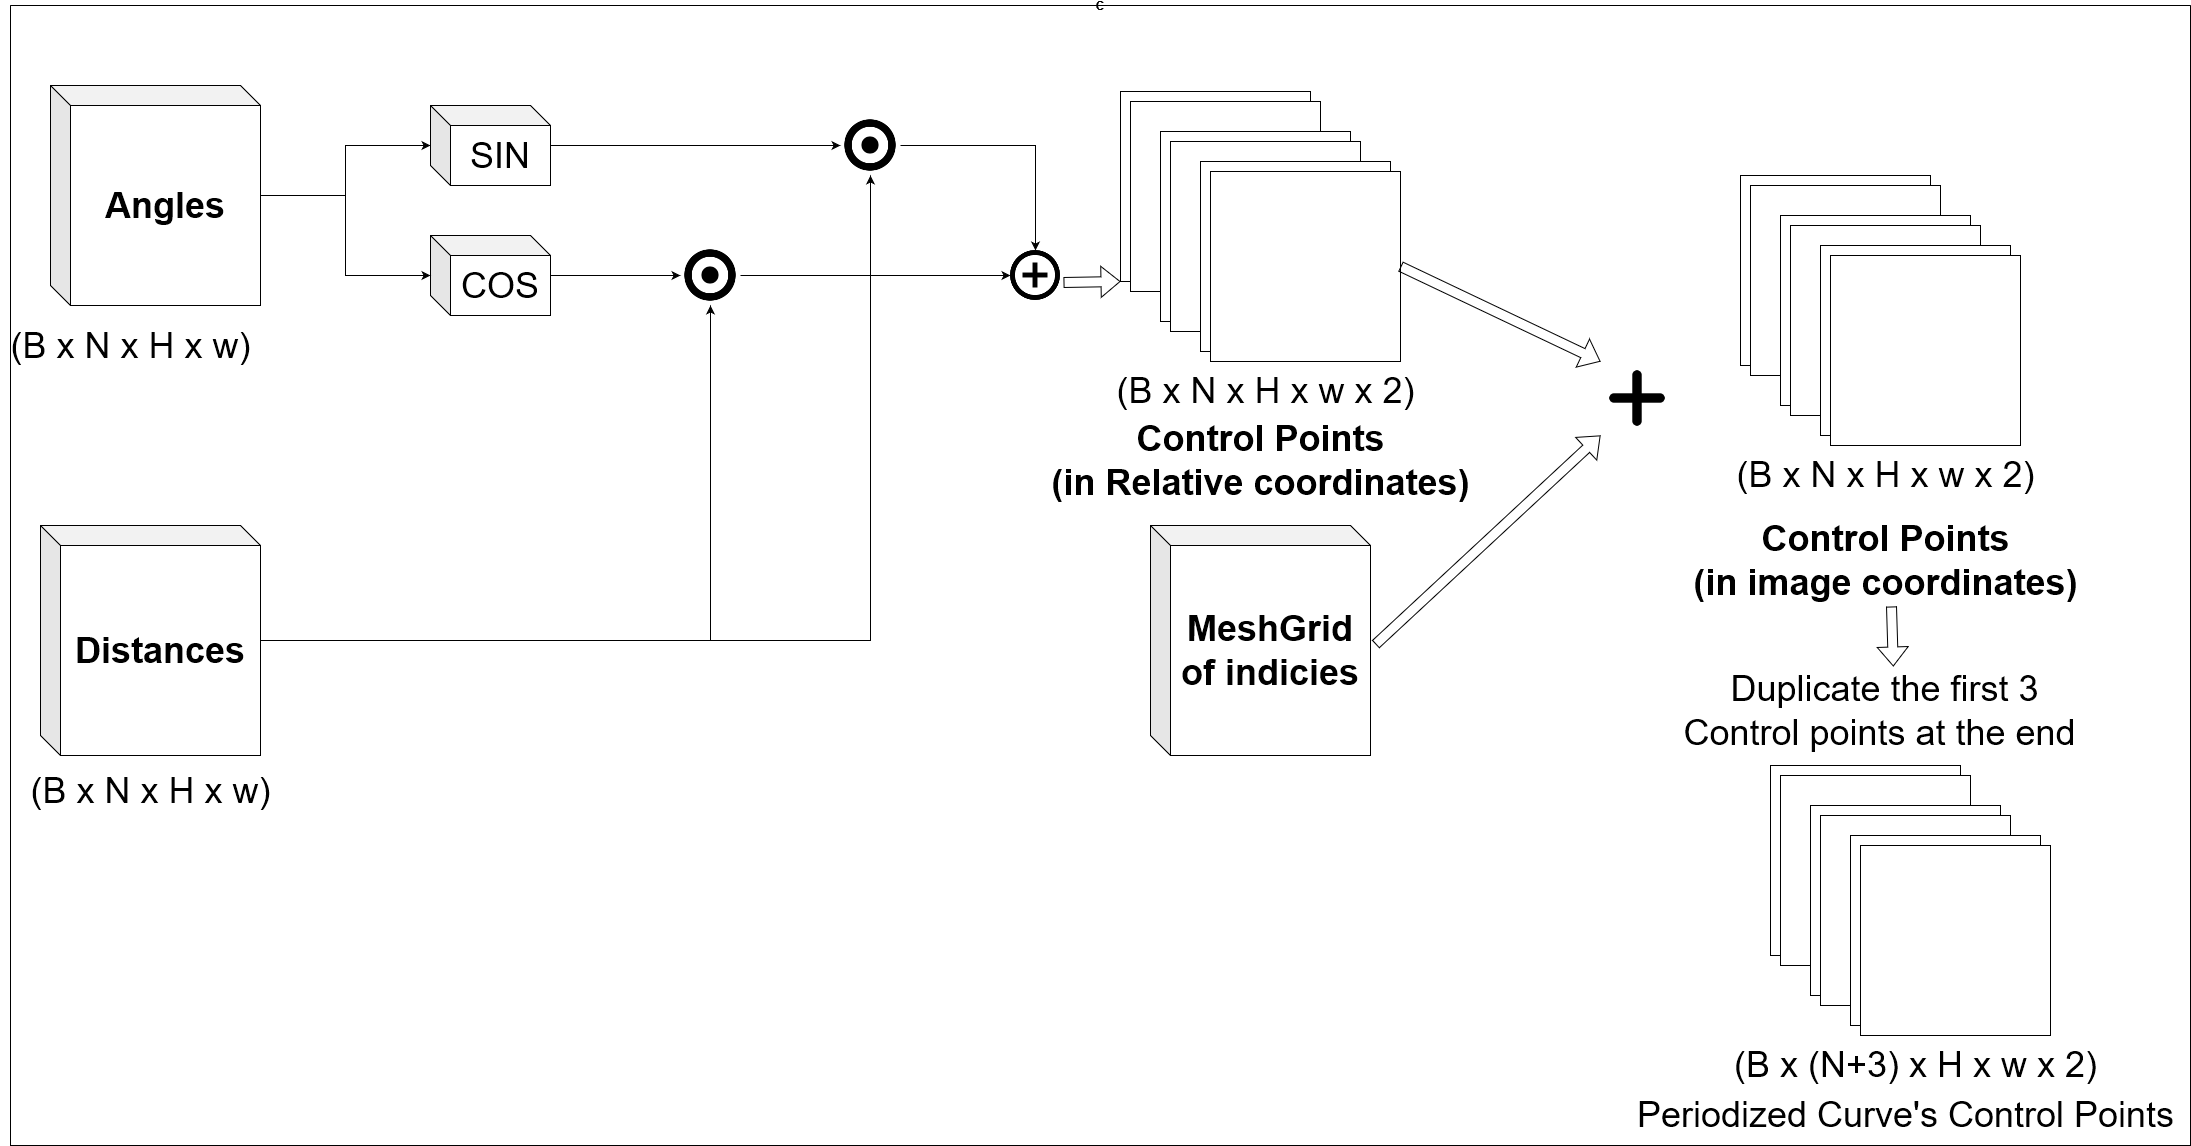
\includegraphics[width=16cm]{presentationImages/ControlPoints.png}
    \caption{Control points extraction branch}
\end{figure}


\section{Preprocessing}
Our model requires transforming the ground truth masks to several components.

\begin{figure}[H]
    \centering
    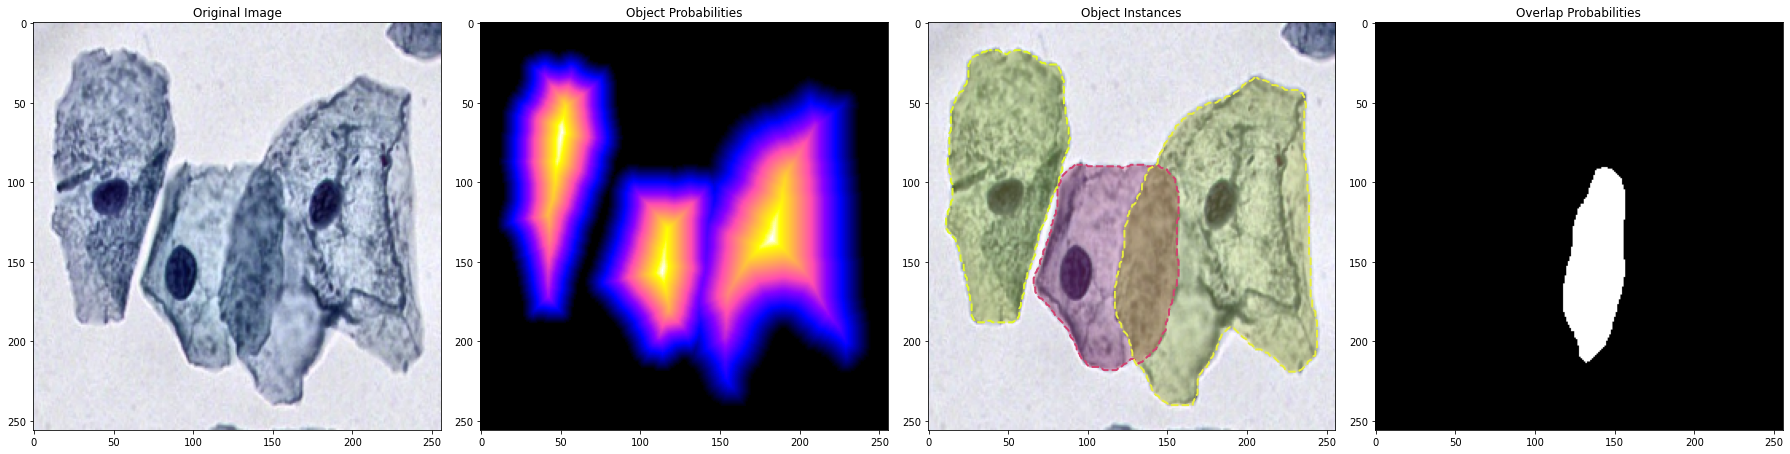
\includegraphics[height=4cm]{presentationImages/overlap.png}
    \caption{Example of the CISD dataset preprocessing of the ground truth labels}
\end{figure}

\subsection{Contour extraction}
To extract the ground truth contour, we apply the border following algorithm to extract the list of contour points coordinates. In order to parallelize our operations using Batches, these contours have to be of the same size. We use an up-sampling approach that linearly interpolates segments linking 2 pixels of the contours in order to have a fixed size of MAX\_LEN.  

\begin{figure}[H]
    \centering
    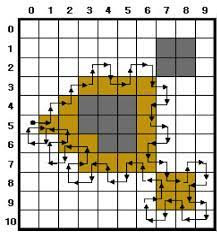
\includegraphics{presentationImages/borderfol.jpg}
    \caption{Pixel following algorithm}
\end{figure}

\subsection{Object probabilities}
To compute the ground truth object probabilities, we apply the normalized euclidean distance transform for each cell instance (measure the distance from the pixels of the cell to the closest point of the background). This has of effect to favor the pixels in the center.These masks are then concatenated using a max operation between all the instances 

\subsection{Overlap probabilities}
For future usages, we would like to extract regions of overlap. These are obtained by summing all the masks together and taking pixels having values greater than 1 (which correspond to overlap) and 0 otherwise.




\section{Postprocessing}
\subsection{Non Maximum Suppresion}
Each pixel of the output image correspond to an object instance, therefore detecting the same object multiple times, in order to get a single prediction for each object We use typical non maximum suppression. where we keep objects with the highest probabilities and suppress the instances that have Intersection Over Union bigger than a certain threshold.

\subsection{Matching instances with the Ground truth}
Once we have a final objects predictions, we match it with the ground truth objects, we define True Positives as objects having IoU over some threshold, False Negative objects in ground truth that have no correspondence, False positive objects in prediction that have no correspondence in the ground truth.
\section{Metrics}
\subsection{Distance Between two instances}
We model the problem as a binary assignment problem, where each pixel from the first contour has a single unique matching from the second.\\

The linear sum assignment problem is also known as minimum weight matching in bipartite graphs. A problem instance is described by a matrix C, where each $C_{ij}$ is the cost of matching vertex i of the first part set (a “worker”) and vertex j of the second set (a “job”). The goal is to find a complete assignment of workers to jobs of minimal cost.\\

Formally, let X be a boolean matrix where 
\begin{equation}
    X_{i,j}=\left\{
                \begin{array}{ll}
                  1 \quad\quad \textit{if row i is assigned to column j}\\
                  0 \quad\quad else
                \end{array}
              \right.
\end{equation}
Then the optimal assignment has cost
\begin{equation}
    \min \sum_i \sum_j C_{ij}X_{ij}
\end{equation}

Each row is assignment to at most one column, and each column to at most one row. The method used is the Hungarian algorithm, also known as the Munkres or Kuhn-Munkres algorithm.

\begin{figure}[H]
    \centering
    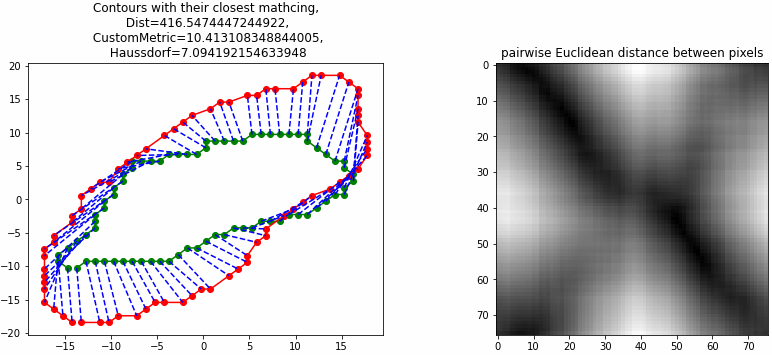
\includegraphics[width=16cm]{images/contourMatching.PNG}
    \caption{Exemple of the matching between pixels from the first contour ans the second contour}
\end{figure}

But this approach -Despite giving the "real" optimal distance between two instances is very slow especially for a large number of instances-. so we use rather simplistic approach, which consist on computing the mean average error

\section{Loss formulation}
Although the definition of the loss may look straightforward, during the Contour loss a matching step is required in order to compute the difference between the expected contour and the target. Except this operation is extremely slow as we have to unpack and iterate each contour individually. To solve this problem, we define a tensor having the same shape as the predicted contours (B x H x W x N x 2), and for all the pixels contained in that particular instance's mask we duplicate the same ground truth contour. relieving the need of a matching phase, and allowing direct computation of the absolute mean error.
% \begin{equation}
    
% \end{equation}
\section{Evaluation}
To evaluate the performance of the detection, we use the Average precision Metric. by using several confidence threshold (Intersection over union with the ground truth) we can observe the behavior of our model in detail. We draw for each confidence level a precision recall curve showcasing the potential of the model with multiple Object probabilities (allowing to pick an optimal threshold as well)



\end{document}


